\startfirstchapter{Introduction}
\label{chapter:introduction}

Semantics is the branch of linguistics which is concerned with the study of language and how we understand the meaning of words and concepts. Cognitive Psychologists study semantics to understand various mechanisms that are involved in the thought process and mental representations which are fundamental to any language. 
Over the recent years, several studies have been performed to understand the similarities between semantic features across different representations such as the brain, image and text. The results from these studies have significant implications in the field of Computation Linguistics and Artificial Intelligence (AI). For example study of the semantics of image features could help us build better computer systems that are capable of performing object recognition such as those used in self-driving cars. 

Distributional Semantic (DS) models or word vectors are based on the occurrence of words in large corpora of text. The main intuition behind these models is that words which are used in the same context in texts could have some similarities with each other. In these semantic models, the meaning of a word is represented by a vector which approximates the relative position of a word in a large high dimensional space. The words which are used in the same context and thus have similar meaning are positioned closer to one another in the vector space. Its vital to perform evaluation of these word vectors since their usage is widely spread across the field of AI. Some of the popular DS models are discussed under chapter \ref{chapter:problem} of this thesis.

\section{The Study of Human Brain}
Computational linguists have also adopted semantic models based on text to study semantic representations in the human brain. The study of the human brain helps us to gain knowledge about how language is processed and interpreted by us. Over the last decade, we have made significant progress in unlocking the complex process through which our brain decodes and understands the meaning of various concepts. This could be credited to the development of various brain imaging techniques such as Functional Magnetic Resonance Imaging (fMRI), Electro-Encephalogram (EEG), Magnetoencephalography (MEG) etc. Linguists studying the brain often use Distributed Semantic models as ground truth in their research.


The inception of such studies began with Mitchell et al. (2008) who were the first to use text-based DS models to study semantic features of concepts in human brain collected using fMRI \cite{Mitchell1191}. They showed that a computational model trained on text corpora could predict neural patters of participants recorded using fMRI.  Murphy et al. (2009) showed that text-based language models could predict EEG activity related to semantics~\cite{MurphyEEG}. This was followed by Sudre et al. (2012) who performed similar work using MEG data collected from subjects viewing images of concrete nouns \cite{SUDRE2012451}.  They also evaluated the performance of various corpus-based models on their task. These works indicate that the semantic representation extracted from corpus could contribute to the study of the brain. 

\section{Introduction to BrainBench}
Anderson et al. argued that a strong correlation between the neural signal and corpus-based models \cite{Mitchell1191, MurphyEEG, SUDRE2012451} is a good indicator that brain data could be used to test corpus-based models \cite{andersonBrainEyes}. If a corpus-based model could approximate and predict the semantic feature representation in the brain, then that model could have features that represents how humans learn and understand language. Similar arguments were made by Murphy et al. (2012) \cite{Murphy2012} and Anderson et al. (2015) \cite{Anderson2015}. Based on these recommendations, Xu et al. (2016) introduced \textit{BrainBench}: a system designed to test corpus-based distributional models of semantics using brain data \cite{BrainBench2016}. 

BrainBench used two brain image datasets: a fMRI dataset \cite{Mitchell1191} and a MEG dataset \cite{SUDRE2012451} collected from nine participants imagining 60 concrete nouns. \textit{``Concrete nouns (e.g. Car, Apple etc.) are things which can be experienced by the five senses whereas abstract nouns are intangible concepts such as ideas and emotions (e.g. freedom, happy)''}~\cite{wiki:xxx}. They tested six popular word vector models against fMRI and MEG datasets and reported comparable performance to other systems which evaluate and benchmark DS models based on behavioral data. Another notable feature of BrainBench was that it is fast and computationally cheap. 

However, BrainBench tests include just 60 concrete nouns, and does not include any abstract nouns. This could imply that the BrainBench tests could be more biased towards word vectors which has a higher distribution of concrete nouns over abstract. Moreover, the tests are derived from only two dataset sources and based on one language (English). This thesis aims to address some of the above limitations of BrainBench.
\bigbreak

\noindent \textbf{The contributions made to BrainBench (\textit{Contribution A}) by this thesis are addressed below:}

\begin{itemize}

\item{Addition of an Italian fMRI brain data into BrainBench and study of the performance of non-English word vectors.}

\item {Introduction of abstract nouns into the BrainBench tests and evaluation of the performance of various word vectors on abstract nouns compared to concrete nouns.}

\item {Addition of an EEG dataset to BrainBench}

\item {The integration into Brainbench the ability to study the performance of word vectors across anatomical brain regions.}

\item{ An increase in the coverage of concepts supported by BrainBench from 60 to 190 concepts}.
\end{itemize}
%summarized in the section \textit{problem statements} of this chapter.

\section{Learning semantics from Images}
BrainBench and other works are based on the study of semantics in the human brain which could improve our understanding of how we learn and interpret languages. Humans also learn semantics from visual input (sight). In fact, there has been research done to show that our first exposure to the semantics is through the visual stimulus captured by our eyes~\cite{norton2007through}. Looking at images, we can recognize content, derive semantics, and sometimes images may even elicit an emotional response in us. It is the human visual cortex that helps us to interpret these visual stimuli and derive semantics from our sight.  

Today, we have Artificial Intelligence (AI) which can recognize objects from images. Most popular of these AI is the Convolutional Neural Network (CNN) which is a type of Artificial Neural Network (ANN) loosely inspired by the human visual cortex. CNNs has importance in many areas of science. Self-driving cars use CNNs as their eyes on the road. Astronomers use CNNs to identify planets and stars from the millions of images taken by telescopes across the world. Doctors and diagnosticians use CNNs to study medical images and predict life-threatening diseases like cancer in patients. Its applications are limitless and ubiquitous. 

Researchers strongly believe that CNNs and deep learning are the future of AI. Yet, we cannot currently explain why these networks work so well, sometimes even better than us humans at various tasks. Could we trust an AI to do our daily tasks if we don't understand its decisions or how it is working?


%The black box nature of Convolutional Nets
\subsection{Black-Box nature of Convolutional Neural Networks}

Researchers in the field of computer vision have created deeper and more complex CNN architectures in search of improved accuracies at the task of object recognition. This trend of going deeper with CNNs has lead to the creation of a myriad of black box architectures which works well at the task of object classifications. Yet, there is a lack of understanding about why they perform so well or how could they be improved \cite{CNNVisual1}. There has been some interest in the computer vision community to provide insights into the performance of these networks. Such insights could help us to train faster and more robust CNNs. \textit{How do Convolutional Networks see the world? What are the features learned by these networks? What makes one network architecture better than the other?} These are some of the questions asked by the deep learning community.

Researchers have focused on methods such as visualization of features of different layers of CNN \cite{CNNVisual1, CNNVisual2, CNNVisual3} or even mathematical models \cite{CNNVisual4} to understand and explain the predictions of CNNs. However, in this thesis, we propose a novel method to understand CNNs by studying the semantic representation through the layers of CNNs. Convolutional Neural Networks might learn semantics from the images, and we believe that the features learned by the CNN could correlate with the semantics of the image. We, therefore, propose that studying the semantic representation instead of feature representation through the layers of CNN could provide us with other valuable insights. 

\begin{figure}[t]
\centering
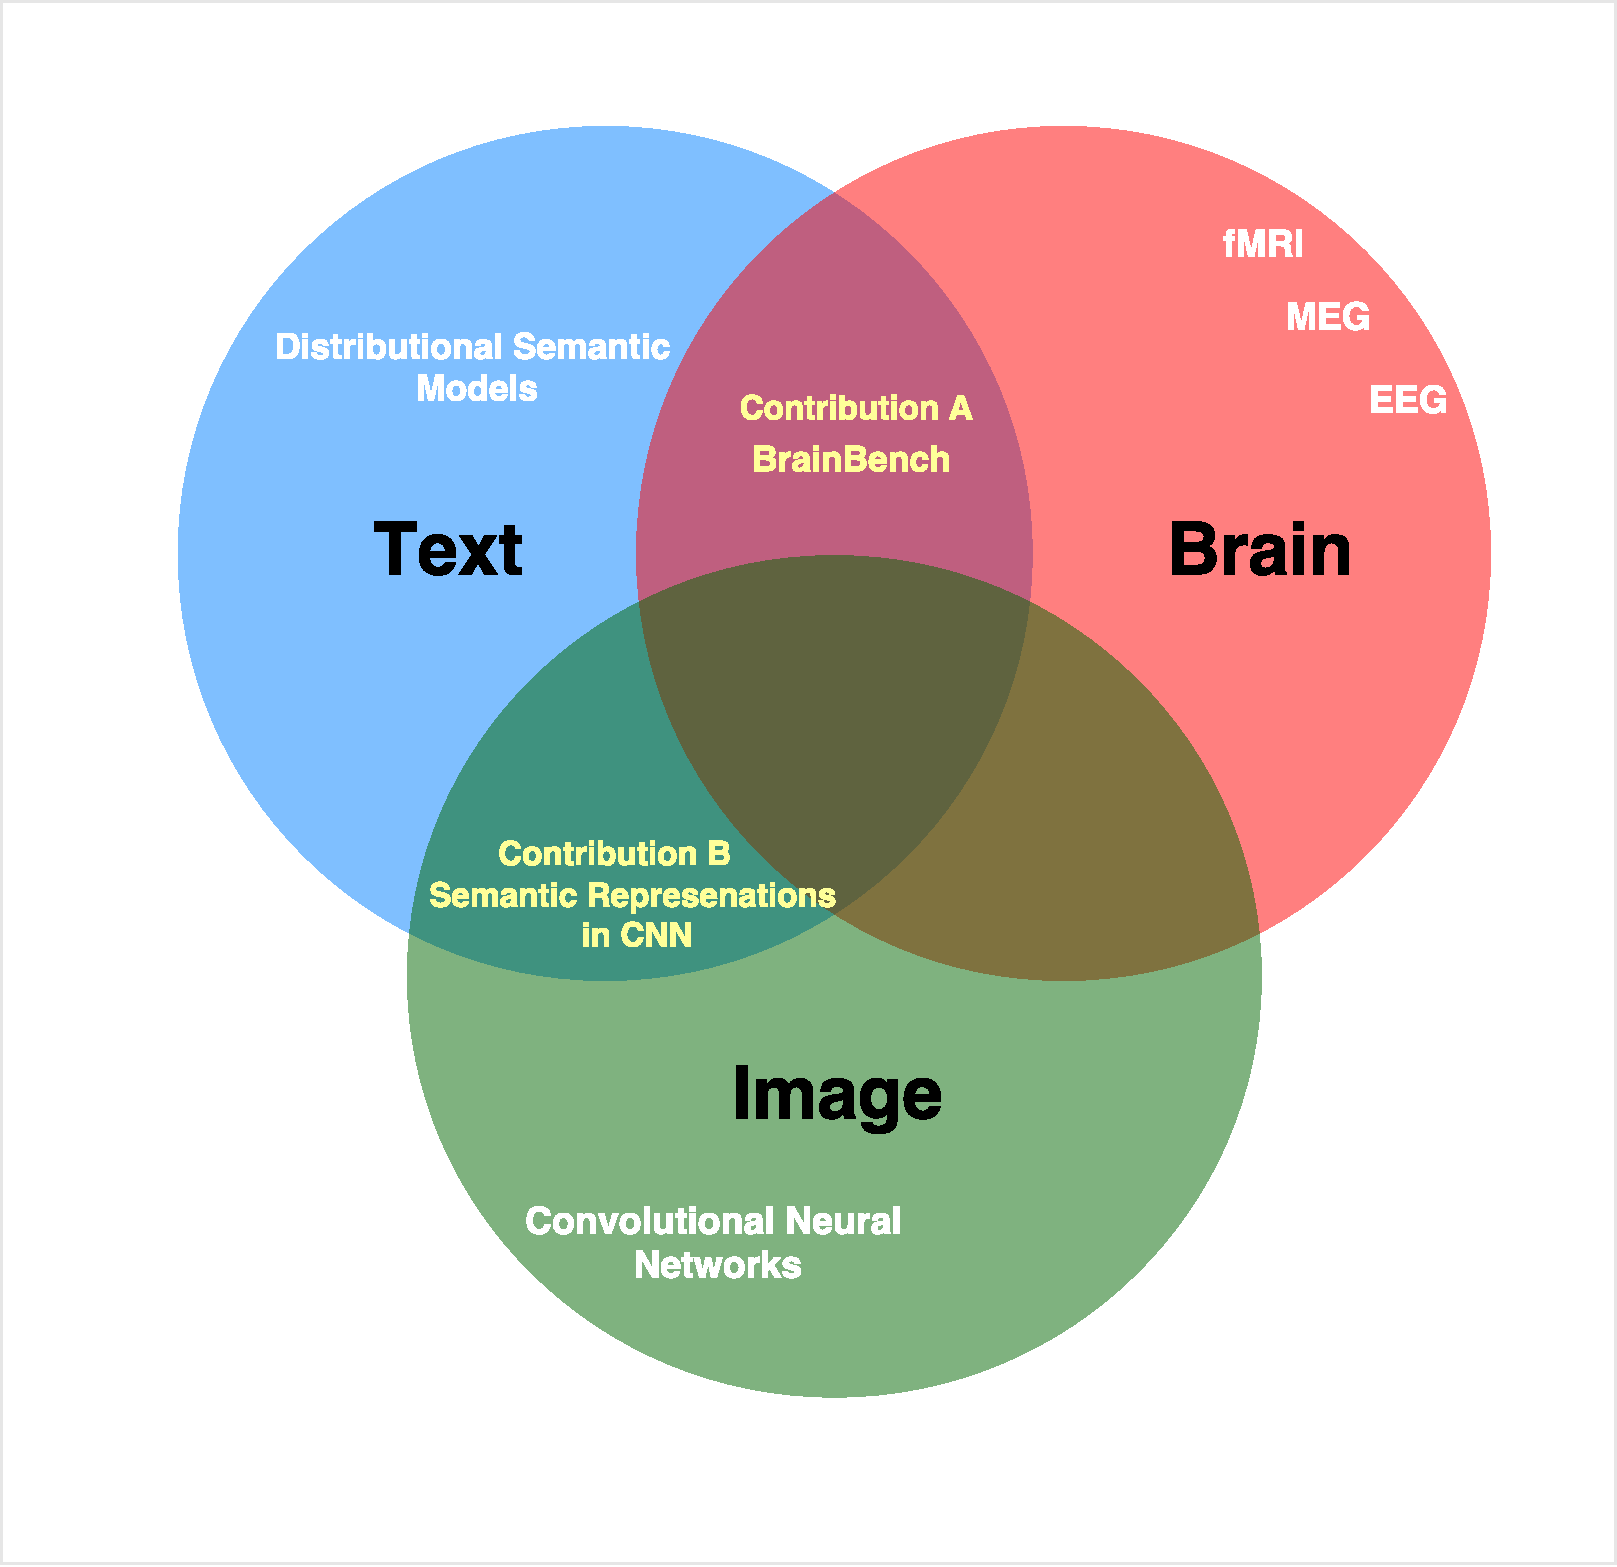
\includegraphics[width=9cm, height=8cm]{Figures/semantics}
\caption{ Representations of Semantics highlighting contributions of this thesis}
\label{Representations}
\end{figure} 

The convergence of semantic information in these networks could be studied with the help of word vectors following the same methodologies used to study semantics in human brain~\cite{Mitchell1191, MurphyEEG, SUDRE2012451}. The study of semantic representation through the layers of CNN could help us understand how various CNN architectures differ from one another and could potentially provide us with a methodology to improve them. Research has shown that a CNN does learn abstract features from images~\cite{CNNVisual1} but does it understand semantics from the images that it's trained on? If a CNN does understand semantics, could we then use that knowledge to explain the decisions made by these networks and unlock the black box?

CNNs are trained on images, and  DS models are trained on the text. Yet they could share a similar semantic representation since they are modeling the same real-world concepts. Studying semantic representations in CNNs could contribute to better understanding of CNNs and potentially pave the way for improved design and debugging of CNNs. To demonstrate an application, we also conduct experiments to determine the position in the hierarchy of the CNN where misclassifications of images could occur.
\bigbreak
\noindent \textbf{The contributions made by this thesis to understand CNNs  (\textit{Contribution B}) are summarized below:}
\begin{itemize}
\item{A novel methodology to study semantic representation through hierarchical layers of CNN.}
\item{The study of hidden representations of images that are misclassified.}
\end{itemize}
% %Problem statements
% \section{Problem Statement}
% In this section, we summarize the problem statements addressed by this thesis. We also elucidate the contributions made by this work to address these gaps in research.

% This chapter introduced \textit{BrainBench}- a system designed to test corpus-based distributional models of semantic using brain data \cite{BrainBench2016}. The system reported comparable performance to other systems which evaluate and benchmark DSM's. Another notable feature of BrainBench was that it is fast and computationally cheaper as compared to other existing methods. It is also made available as a web-service which makes it useful for practical applications.

% However, so far BrainBench tests include just 60 concrete nouns.  Nouns only form a small subset of various parts of speech that constitutes the language. Another limitation is that the tests do not include any abstract nouns. This could imply that the BrainBench tests could be more biased towards word vectors that has a higher distribution of concrete nouns over abstract. Moreover, the tests are derived from only two dataset sources (a fMRI and a MEG) and based on one language (English). Considering that DSM's are available in multiple languages and not including brain data from other language sources as a part of BrainBench tests is a limitation.
% \bigbreak









\section{Thesis Organization}

\begin{description}
\item[\textbf{Chapter 1}] includes a brief introduction to the world of semantics; it's various representations and description of the problem statements.
\item[\textbf{Chapter 2}] talks about related work in this area of research and provides a detailed walkthrough of all the major contributions made in this field. 
\item[\textbf{Chapter 3}] talks about contributions made to BrainBench including the addition of two new datasets and study of semantic features within various regions of human brain. The results of these experiments along with the discussions are also included in this chapter.
\item[\textbf{Chapter 4}] describes the study of semantic representations through the layers of popular convolutional neural networks with results and discussions.
\item[\textbf{Chapter 5}] gives a summary of the problem statements and the contribution of this thesis in solving those problems. We also discuss various future improvements in this area of research.
\end{description}